
%-------------------------------------------------%
% Atividade Prática 5 - Design Patterns (Observer)
%-------------------------------------------------%
\documentclass[aspectratio=169]{beamer}

\usepackage[english,brazil]{babel}
\usepackage[style=abnt,noslsn,justify]{biblatex}
\renewcommand*{\bibfont}{\small}
\usepackage{csquotes}
\addbibresource{referencias_trabalho.bib}

\usepackage{listings}
\lstset{
  basicstyle=\ttfamily\scriptsize,
  keywordstyle=\bfseries\color{blue!70!black},
  commentstyle=\itshape\color{gray},
  stringstyle=\color{orange!80!black},
  breaklines=true,
  showstringspaces=false,
  tabsize=2,
  frame=single,
  numbers=left,
  numberstyle=\tiny\color{gray},
  xleftmargin=1.5em,
  framexleftmargin=1.5em,
}

\definecolor[named]{novaCor}{HTML}{303A52}
\definecolor{azul-seg}{RGB}{27, 85, 142}

% Theme parameters
\usetheme[
    foreground=azul-seg,
]{ifsclean}

% -------------------------------------------------%
%              Título
% -------------------------------------------------%
\title{Observer}
\subtitle{Atividade Prática 5 -- Design Patterns}
\author{
  Nicolas Arthur Raulino Oliveira
}
\institute{Instituto Federal de Santa Catarina}
\date{Abril de 2026}

% -------------------------------------------------%
\begin{document}

\begin{frame}[plain, noframenumbering]
    \maketitle
\end{frame}

\begin{frame}[plain, noframenumbering]{Licenciamento}
    \licenciamentoLivre
\end{frame}
% -------------------------------------------------%
\begin{frame}[plain, noframenumbering]{Sumário}
    \tableofcontents
\end{frame}

% -------------------------------------------------%
\section{Nome e Tipo}
% -------------------------------------------------%

\begin{frame}{Observer -- Padrão Comportamental}
    \begin{itemize}
        \item \textbf{Nome}: Observer (Observador)
        \item \textbf{Tipo}: Padrão Comportamental
        \item \textbf{Definição}: permite definir um mecanismo de assinatura para notificar múltiplos objetos sobre quaisquer eventos que aconteçam com o objeto que eles estão observando.
    \end{itemize}
\end{frame}

% -------------------------------------------------%
\section{Problema}
% -------------------------------------------------%

\begin{frame}{O Problema}
    Imagine dois objetos: um \textbf{Cliente} e uma \textbf{Loja}.

    \vspace{0.5em}
    O cliente quer saber quando um novo produto estará disponível.

    \begin{itemize}
        \item \textbf{Opção 1}: o cliente visita a loja todos os dias -- maioria das visitas em vão.
        \item \textbf{Opção 2}: a loja envia e-mails para \emph{todos} os clientes -- spam para quem não tem interesse.
    \end{itemize}

    \begin{figure}
        \centering
        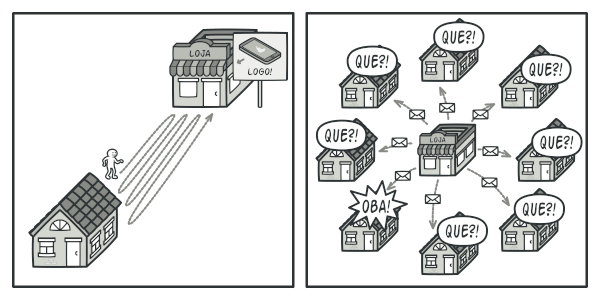
\includegraphics[width=0.55\linewidth]{img/img-1.png}
    \end{figure}
\end{frame}

% -------------------------------------------------%
\section{Solução}
% -------------------------------------------------%

\begin{frame}{Como o Observer Resolve}
    \begin{itemize}
        \item O objeto com estado interessante é a \textbf{Publicadora} (sujeito).
        \item Os objetos interessados são os \textbf{Assinantes} (observadores).
        \item A publicadora mantém uma \textbf{lista de assinantes} e métodos para \texttt{assinar} / \texttt{desassinar}.
        \item Quando um evento ocorre, a publicadora \textbf{notifica todos os assinantes}.
    \end{itemize}

    \begin{figure}
        \centering
        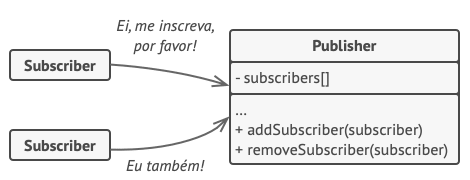
\includegraphics[width=0.5\linewidth]{img/img-2.png}
    \end{figure}
\end{frame}

\begin{frame}{Interface Comum}
    \begin{columns}
        \begin{column}{0.45\textwidth}
            \begin{itemize}
                \item Todos os assinantes implementam a \textbf{mesma interface} (ex: método \texttt{atualizar}).
                \item A publicadora se comunica \textbf{apenas através dessa interface}.
                \item Isso evita \textbf{acoplamento} entre a publicadora e as classes concretas dos assinantes.
            \end{itemize}
        \end{column}
        \begin{column}{0.52\textwidth}
            \begin{figure}
                \centering
                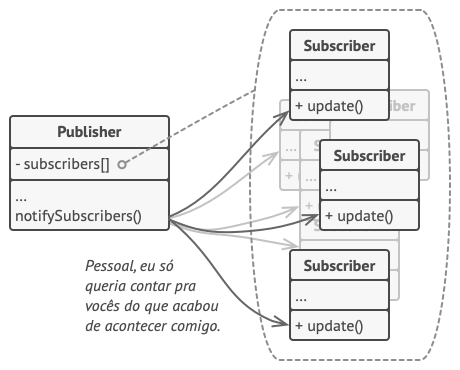
\includegraphics[width=\linewidth]{img/img-3.png}
            \end{figure}
        \end{column}
    \end{columns}
\end{frame}

\begin{frame}{Analogia: Assinatura de Jornal}
    \begin{columns}
        \begin{column}{0.45\textwidth}
            \begin{itemize}
                \item Você \textbf{assina} um jornal e recebe novas edições automaticamente.
                \item Não precisa ir à banca verificar.
                \item Pode \textbf{cancelar} a assinatura a qualquer momento.
            \end{itemize}
        \end{column}
        \begin{column}{0.5\textwidth}
            \begin{figure}
                \centering
                
\includegraphics[width=\linewidth]{img/img-4.png}
            \end{figure}
        \end{column}
    \end{columns}
\end{frame}

% -------------------------------------------------%
\section{Estrutura}
% -------------------------------------------------%

\begin{frame}{Diagrama de Estrutura}
    \begin{figure}
        \centering
        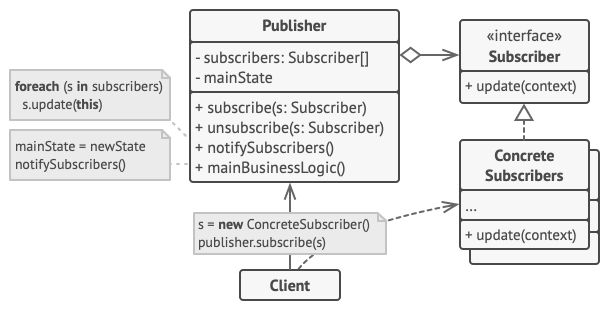
\includegraphics[width=0.75\linewidth]{img/img-5.png}
    \end{figure}
\end{frame}

\begin{frame}{Componentes do Diagrama}
    \begin{enumerate}
        \item \textbf{Publicadora}: mantém lista de assinantes e envia notificações.
        \item \textbf{Interface Assinante}: declara o método \texttt{atualizar}.
        \item \textbf{Assinantes Concretos}: reagem às notificações, implementando a interface.
        \item \textbf{Cliente}: cria publicadoras e registra assinantes.
    \end{enumerate}

    \vspace{0.5em}
    A publicadora pode passar \textbf{dados de contexto} junto à notificação, ou passar a si mesma como argumento.
\end{frame}

% -------------------------------------------------%
\section{Exemplo}
% -------------------------------------------------%

\begin{frame}{Exemplo: Editor de Texto}
    Um editor de texto notifica serviços sobre mudanças em seu estado.

    \begin{figure}
        \centering
        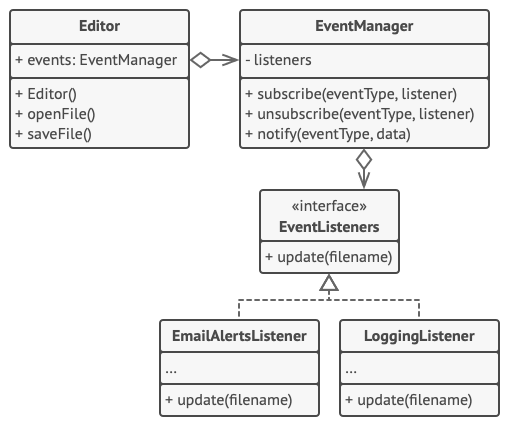
\includegraphics[width=0.50\linewidth]{img/img-6.png}
    \end{figure}

    \vspace{-0.5em}
    \begin{itemize}
        \item O editor \textbf{delega} o gerenciamento de assinaturas a um \texttt{EventManager}. Assinantes podem começar ou parar de ouvir \textbf{dinamicamente}.
    \end{itemize}
\end{frame}

\begin{frame}[fragile]{Código Java -- Interface Observer}
\begin{lstlisting}[language=Java,title={Interface Observer}]
interface Observer {
    void update(String message);
}
\end{lstlisting}
\end{frame}

\begin{frame}[fragile]{Código Java -- Publisher}
\begin{lstlisting}[language=Java,title={Publisher (Subject)}]
class Publisher {
    private List<Observer> observers = new ArrayList<>();

    public void subscribe(Observer o) {
        observers.add(o);
    }

    public void unsubscribe(Observer o) {
        observers.remove(o);
    }

    public void notifyObservers(String message) {
        for (Observer o : observers) {
            o.update(message);
        }
    }
}
\end{lstlisting}
\end{frame}

\begin{frame}[fragile]{Código Java -- Observadores Concretos}
\begin{lstlisting}[language=Java,title={Observadores concretos}]
class EmailSubscriber implements Observer {
    public void update(String message) {
        System.out.println("Email recebido: " + message);
    }
}

class SmsSubscriber implements Observer {
    public void update(String message) {
        System.out.println("SMS recebido: " + message);
    }
}
\end{lstlisting}
\end{frame}

\begin{frame}[fragile]{Código Java -- Aplicação}
\begin{lstlisting}[language=Java,title={Uso no main}]
public class Main {
    public static void main(String[] args) {
        Publisher loja = new Publisher();

        Observer cliente1 = new EmailSubscriber();
        Observer cliente2 = new SmsSubscriber();

        loja.subscribe(cliente1);
        loja.subscribe(cliente2);

        loja.notifyObservers("Novo produto disponivel!");
    }
}
\end{lstlisting}
\end{frame}

% -------------------------------------------------%
\section{Vantagens e Desvantagens}
% -------------------------------------------------%

\begin{frame}{Vantagens e Desvantagens}
    \begin{columns}[T]
        \begin{column}{0.48\textwidth}
            \textbf{Vantagens}
            \begin{itemize}
                \item \textbf{Princípio Aberto/Fechado}: novas classes assinantes sem alterar a publicadora.
                \item \textbf{Relações dinâmicas}: assinantes podem entrar e sair durante a execução.
            \end{itemize}
        \end{column}
        \begin{column}{0.48\textwidth}
            \textbf{Desvantagens}
            \begin{itemize}
                \item Assinantes são notificados em \textbf{ordem aleatória}.
            \end{itemize}
        \end{column}
    \end{columns}
\end{frame}

% -------------------------------------------------%
\begin{frame}[allowframebreaks]{Referências}
    \nocite{*}
    \printbibliography
\end{frame}

\end{document}
